%%%%%%%%%%%%%%%%%%%%%%%%%%%%%%%%%%%%%%%%%
% Arsclassica Article
% LaTeX Template
% Version 1.1 (1/8/17)
%
% This template has been downloaded from:
% http://www.LaTeXTemplates.com
%
% Original author:
% Lorenzo Pantieri (http://www.lorenzopantieri.net) with extensive modifications by:
% Vel (vel@latextemplates.com)
%
% License:
% CC BY-NC-SA 3.0 (http://creativecommons.org/licenses/by-nc-sa/3.0/)
%
%%%%%%%%%%%%%%%%%%%%%%%%%%%%%%%%%%%%%%%%%

%----------------------------------------------------------------------------------------
%	PACKAGES AND OTHER DOCUMENT CONFIGURATIONS
%----------------------------------------------------------------------------------------





\documentclass[
10pt, % Main document font size
a4paper, % Paper type, use 'letterpaper' for US Letter paper
oneside, % One page layout (no page indentation)
%twoside, % Two page layout (page indentation for binding and different headers)
headinclude,footinclude, % Extra spacing for the header and footer
BCOR5mm, % Binding correction
]{scrartcl}


\usepackage{listings}
\usepackage{color}

\definecolor{dkgreen}{rgb}{0,0.6,0}
\definecolor{gray}{rgb}{0.5,0.5,0.5}
\definecolor{mauve}{rgb}{0.58,0,0.82}

\lstset{frame=tb,
	language=C,
	aboveskip=3mm,
	belowskip=3mm,
	showstringspaces=false,
	columns=flexible,
	basicstyle={\small\ttfamily},
	numbers=none,
	numberstyle=\tiny\color{gray},
	keywordstyle=\color{blue},
	commentstyle=\color{dkgreen},
	stringstyle=\color{mauve},
	breaklines=true,
	breakatwhitespace=true,
	tabsize=3
}



\usepackage{german}

%usepackage[utf8]{inputenc}
%\usepackage{geometry}
\usepackage[german,onelanguage,linesnumbered, ruled]{algorithm2e}
\SetAlFnt{\small}
\SetAlCapFnt{\large}
\SetAlCapNameFnt{\large}
%\usepackage{algpseudocode}


%%%%%%%%%%%%%%%%%%%%%%%%%%%%%%%%%%%%%%%%%
% Arsclassica Article
% Structure Specification File
%
% This file has been downloaded from:
% http://www.LaTeXTemplates.com
%
% Original author:
% Lorenzo Pantieri (http://www.lorenzopantieri.net) with extensive modifications by:
% Vel (vel@latextemplates.com)
%
% License:
% CC BY-NC-SA 3.0 (http://creativecommons.org/licenses/by-nc-sa/3.0/)
%
%%%%%%%%%%%%%%%%%%%%%%%%%%%%%%%%%%%%%%%%%

%----------------------------------------------------------------------------------------
%	REQUIRED PACKAGES
%----------------------------------------------------------------------------------------

\usepackage[
nochapters, % Turn off chapters since this is an article        
beramono, % Use the Bera Mono font for monospaced text (\texttt)
eulermath,% Use the Euler font for mathematics
pdfspacing, % Makes use of pdftex’ letter spacing capabilities via the microtype package
dottedtoc % Dotted lines leading to the page numbers in the table of contents
]{classicthesis} % The layout is based on the Classic Thesis style

\usepackage{arsclassica} % Modifies the Classic Thesis package

\usepackage[T1]{fontenc} % Use 8-bit encoding that has 256 glyphs

\usepackage[utf8]{inputenc} % Required for including letters with accents

\usepackage{graphicx} % Required for including images
\graphicspath{{Figures/}} % Set the default folder for images

\usepackage{enumitem} % Required for manipulating the whitespace between and within lists

\usepackage{lipsum} % Used for inserting dummy 'Lorem ipsum' text into the template

\usepackage{subfig} % Required for creating figures with multiple parts (subfigures)

\usepackage{amsmath,amssymb,amsthm} % For including math equations, theorems, symbols, etc

\usepackage{varioref} % More descriptive referencing

%----------------------------------------------------------------------------------------
%	THEOREM STYLES
%---------------------------------------------------------------------------------------

\theoremstyle{definition} % Define theorem styles here based on the definition style (used for definitions and examples)
\newtheorem{definition}{Definition}

\theoremstyle{plain} % Define theorem styles here based on the plain style (used for theorems, lemmas, propositions)
\newtheorem{theorem}{Theorem}

\theoremstyle{remark} % Define theorem styles here based on the remark style (used for remarks and notes)

%----------------------------------------------------------------------------------------
%	HYPERLINKS
%---------------------------------------------------------------------------------------

\hypersetup{
%draft, % Uncomment to remove all links (useful for printing in black and white)
colorlinks=true, breaklinks=true, bookmarks=true,bookmarksnumbered,
urlcolor=webbrown, linkcolor=RoyalBlue, citecolor=webgreen, % Link colors
pdftitle={}, % PDF title
pdfauthor={\textcopyright}, % PDF Author
pdfsubject={}, % PDF Subject
pdfkeywords={}, % PDF Keywords
pdfcreator={pdfLaTeX}, % PDF Creator
pdfproducer={LaTeX with hyperref and ClassicThesis} % PDF producer
} % Include the structure.tex file which specified the document structure and layout

\hyphenation{Fortran hy-phen-ation} % Specify custom hyphenation points in words with dashes where you would like hyphenation to occur, or alternatively, don't put any dashes in a word to stop hyphenation altogether

%----------------------------------------------------------------------------------------
%	TITLE AND AUTHOR(S)
%----------------------------------------------------------------------------------------

\title{\normalfont\spacedallcaps{Projektaufgabe pixCheckTangle}} % The article title

%\subtitle{Subtitle} % Uncomment to display a subtitle

\author{\spacedlowsmallcaps{Raphael Drechsler}} % The article author(s) - author affiliations need to be specified in the AUTHOR AFFILIATIONS block

\date{} % An optional date to appear under the author(s)

%----------------------------------------------------------------------------------------

\begin{document}

%----------------------------------------------------------------------------------------
%	HEADERS
%----------------------------------------------------------------------------------------

\renewcommand{\sectionmark}[1]{\markright{\spacedlowsmallcaps{#1}}} % The header for all pages (oneside) or for even pages (twoside)
%\renewcommand{\subsectionmark}[1]{\markright{\thesubsection~#1}} % Uncomment when using the twoside option - this modifies the header on odd pages
\lehead{\mbox{\llap{\small\thepage\kern1em\color{halfgray} \vline}\color{halfgray}\hspace{0.5em}\rightmark\hfil}} % The header style

\pagestyle{scrheadings} % Enable the headers specified in this block

%----------------------------------------------------------------------------------------
%	TABLE OF CONTENTS & LISTS OF FIGURES AND TABLES
%----------------------------------------------------------------------------------------

\maketitle % Print the title/author/date block

\setcounter{tocdepth}{2} % Set the depth of the table of contents to show sections and subsections only

\tableofcontents % Print the table of contents

\listoffigures % Print the list of figures

\listoftables % Print the list of tables




%----------------------------------------------------------------------------------------

\newpage % Start the article content on the second page, remove this if you have a longer abstract that goes onto the second page

%----------------------------------------------------------------------------------------
%	INTRODUCTION
%----------------------------------------------------------------------------------------
\section{Problembeschreibung}

Gegeben ist ein quadratisches Raster von n x n Feldern. Jedes der Felder kann schwarz oder weiß gefärbt sein. 
Es ist ein Algorithmus zu implementieren, welcher

\begin{itemize}[noitemsep] % [noitemsep] removes whitespace between the items for a compact look
	\item eine Einfache Eingabe eines solche Rasters erlaubt
	\item als Rechteck zusammenhängende Felder im Raster erkennt 
	\item die resultierenden Rechtecke ausgibt
\end{itemize}

Dabei soll der Algorithmus für die Ausführung auf dem Cluster-System implementiert werden.\\
Anschließend soll mittels Laufzeitmessungen die Effizienz der Parallelisierung betrachtet werden. Dafür ist es erforderlich den Algorithmus als sequentiellen Algorithmus ausführen zu können.

\section{Beschreibung der Implementierung}

Die Implementierung ist in zwei Programmen umgesetzt. 

\begin{itemize}[noitemsep] % [noitemsep] removes whitespace between the items for a compact look
	\item \textit{gridGenerator.c}: Programm zum generieren von \textit{.txt}-Dateien, in denen das Raster gespeichert ist.  
	\item \textit{pixCheckTangle.c}: Programm zur Überprüfung des als \textit{.txt}-Datei übergebenen Rasters auf Rechtecke.
\end{itemize}

In den Folgenden Abschnitten wird die Funktionalität der Programme beschrieben.

\subsection{gridGenerator: Generieren der Files}

Das Programm \textit{gridGenerator.c} wird per mpirun-Befehl über die Konsole aufgerufen.\\

\begin{lstlisting}
mpirun gridGenerator.c [gridfile.txt]
\end{lstlisting}

Wird dabei eine zuvor durch den gridGenerator erzeugte .txt-Datei als Parameter angegeben, kann diese Datei bearbeitet werden. Andernfalls wird eine neue Datei erstellt. Der Programm-Ablauf ist im Folgenden als Nassi-Shneiderman-Diagramm dargestellt.\\
\\Der Vollstädige Code ist im Anhang ab Seite (DRT oder Verweis angeben)... gelistet. 
\pagebreak

\begin{figure}[h]
	\centering 
	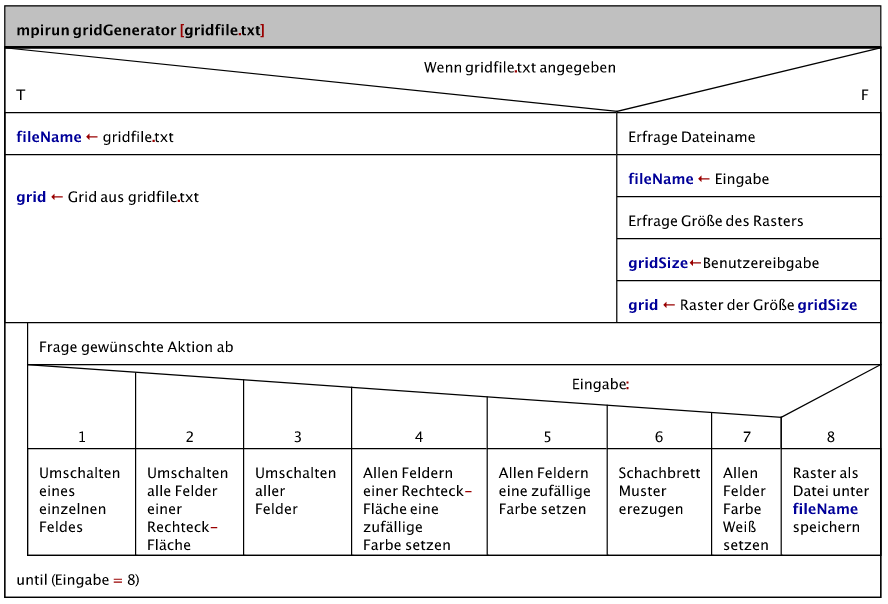
\includegraphics[width=0.9\columnwidth]{Diag_1} 
	\caption[Funktionalität von \textit{gridGenerator.c}]{Funktionalität von \textit{gridGenerator.c} dargestellt als Nassi-Shneiderman-Diagramm}
\end{figure}


\subsection{pixCheckTangle: Beschreibung des Sequentiellen Algorithmus}

Das Programm \textit{pixCheckTangle.c} wird per mpirun-Befehl über die Konsole aufgerufen. Dabei ist als dem Aufruf eine Raster-Textdatei als Argument zu übergeben. Die übergebene Datei wird dann auf Rechtecke überprüft.\\

\begin{lstlisting}
mpirun pixCheckTangle.c gridfile.txt
\end{lstlisting}

Für den Fall, dass nur ein Prozessor an der Ausführung des Programmes beteiligt ist, wird die sequentielle Variante des Algorithmus ausgeführt. Diese ist im Folgenden als BPMN-Daigramm dargestellt.

\begin{figure}[h]
	\centering 
	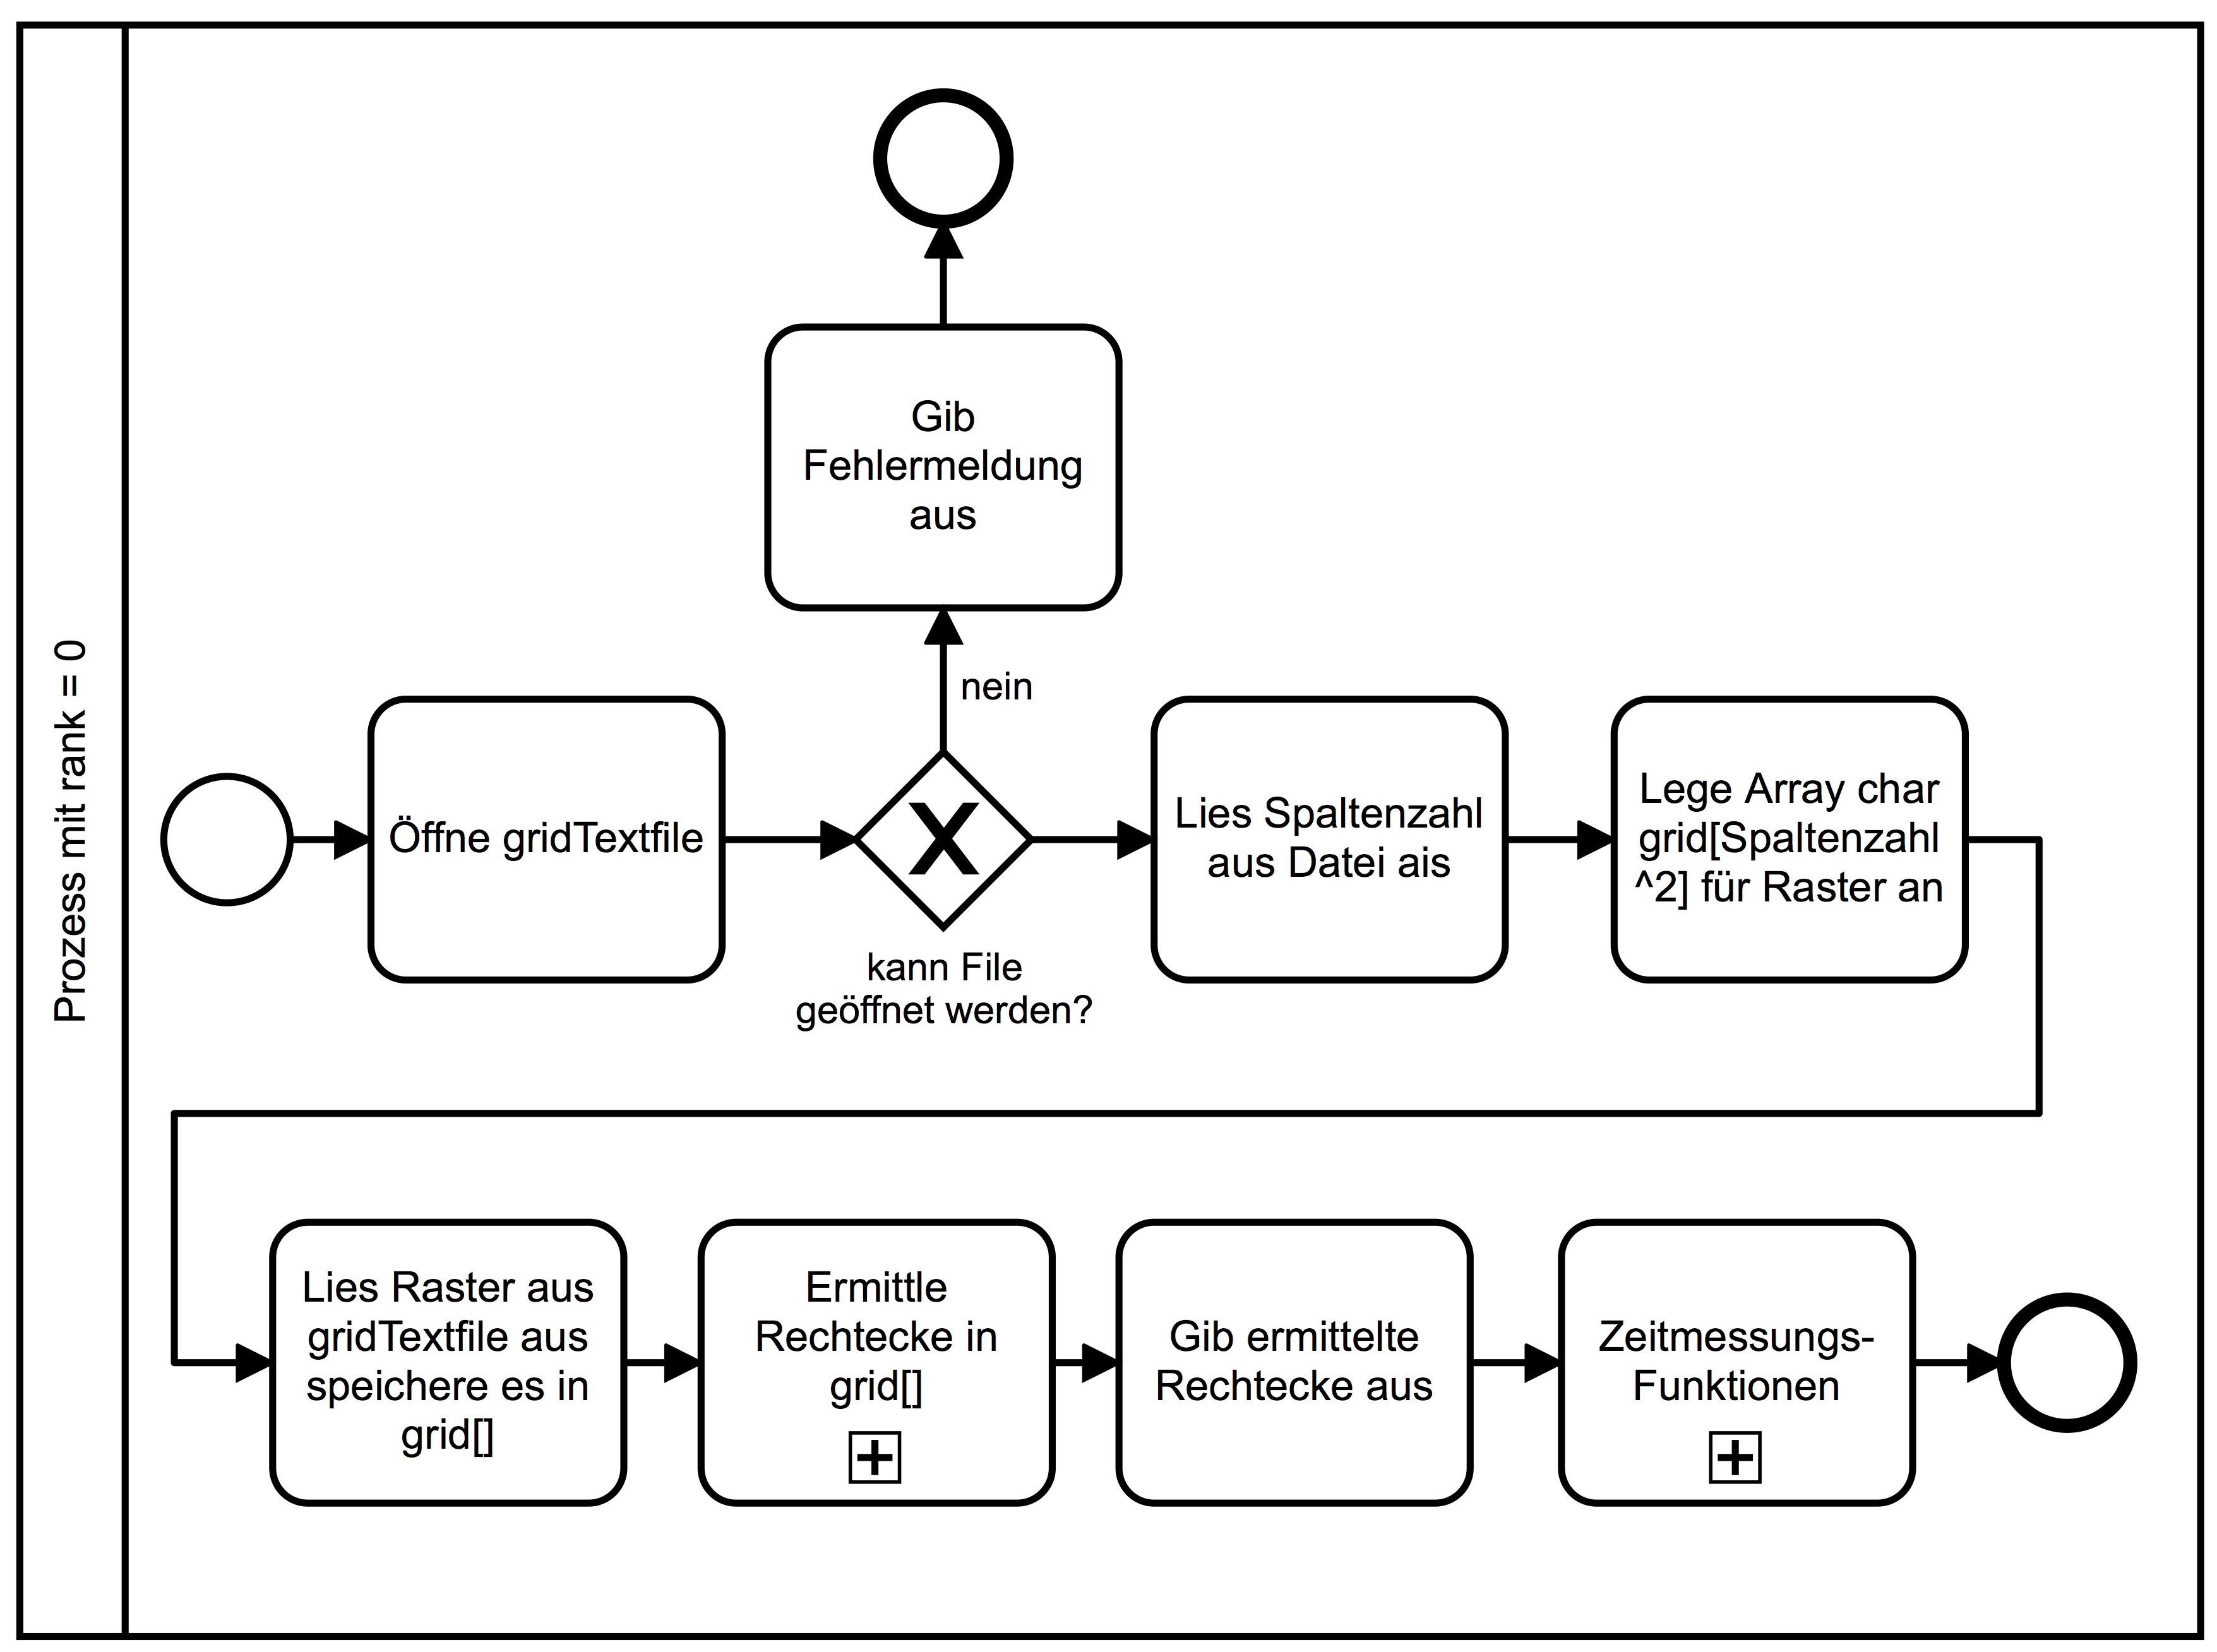
\includegraphics[width=0.8\columnwidth]{Diag_2f} 
	\caption[Funktionalität von \textit{pixCheckTangle.c} sequentiell]{Sequentieller Ablauf von \textit{pixCheckTangle.c} dargestellt als BPMN-Diagramm }
	
\end{figure}

Der vollständige Code zum Algorithmus ist im Anhang enthalten. Die Hauptfunktionalität findet sich dabei in dem Codeabschnitt, welcher ausgeführt wird,   wenn der ausführende Prozess den Rang 0 hat und es nur einen Prozess gibt.
%
%
%\begin{figure}[h]
%	\centering 
%
%	\begin{lstlisting}
%	if(rank == 0){
%			if (noOfProcs==1){
%					//run the sequential porcess
%			} ...
%	\end{lstlisting}
%	\caption[Einordnung \textit{pixCheckTangle.c} sequentiell im Quellcode]{Einordnung des sequentiellen Ablaufs von \textit{pixCheckTangle.c} im Quellcode}
%	
%\end{figure}


Die Funktionalität zum Ermitteln der Rechtecke, wird im Kapitel 2.4 näher beschrieben. Nach welchem Prinzip die Zeitmessung erfolgen, wird in Kapitel 3.1 beschrieben.


\subsection{pixCheckTangle: Beschreibung des Cluster-Algorithmus}

Für den Fall, dass mehrere Prozessoren an der Abarbeitung des Programmes beteiligt sind, wird die Cluster-Variante des Algorithmus ausgeführt.\\
Dabei übernimmt der Prozess mir dem Rang 0 die Rolle des Master-Prozesses. Alle übrigen Prozesse übernehmen die Rolle von Worker-Prozessen. \\
Das Raster wird dann in vom Master-Prozess in mehrere Teile zerlegt. Jeder Worker-Prozess übernimmt dann die Abarbeitung eines Teil-Rasters. \\

\textbf{Beispiel für Verarbeitung durch Cluster-Prozess}

Beispielsweise wird das folgende Raster betrachtet. Das Zeichen \textit{\#} repräsentiert dabei ein schwarzes Feld, weiße Felder werden durch Leerzeichen dargestellt.
\begin{figure}[h]
	\centering 
	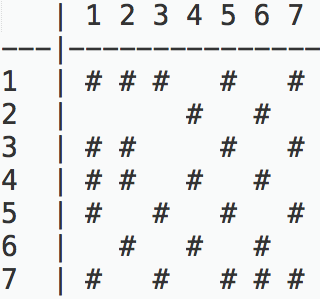
\includegraphics[width=0.25\columnwidth]{Raster_1} 
	\caption[Cluster-Prozess: Beispiel-Raster]{Ein Raster-Beispiel }
\end{figure}

Für den Fall, das an der Abarbeitung des Programmes 4 Prozesse beteiligt sind, wird das Raster vom Master-Prozess in drei Teil-Raster geteilt. Die jeweiligen Teile werden dann den Worker-Prozessen zugewiesen und von diesen abgearbeitet.

\begin{figure}[h]
	\centering 
	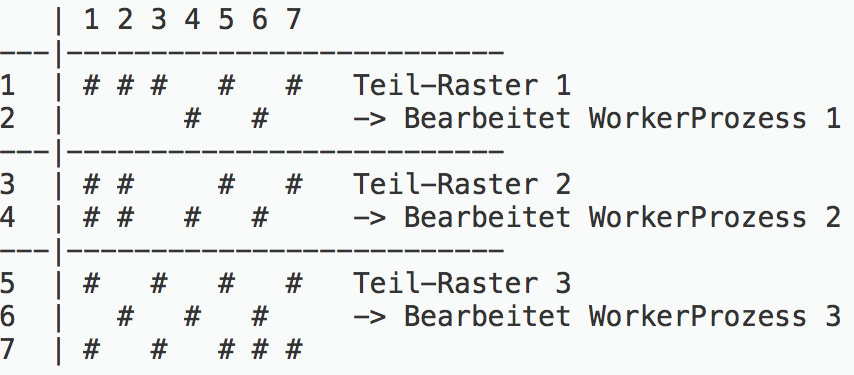
\includegraphics[width=0.6\columnwidth]{Raster_2} 
	\caption[Cluster-Prozess: Aufteilung Beispiel-Raster mit 4 Prozessen]{Aufteilung des Beispiel-Rasters bei 4 Prozessen}
\end{figure}

Die Worker-Prozesse können nun feststellen, ob es sich bei einzelnen/zusammenhängenden Pixeln (im Folgenden als Figur bezeichnet) um Rechtecke handelt oder nicht. In der Folgenden Grafik, werden Figuren, die kein Rechteck darstellen mit einem \textit{X} dargestellt. Rechtecke werden weiterhin durch das Zeichen \textit{\#} repräsentiert.

\begin{figure}[h]
	\centering 
	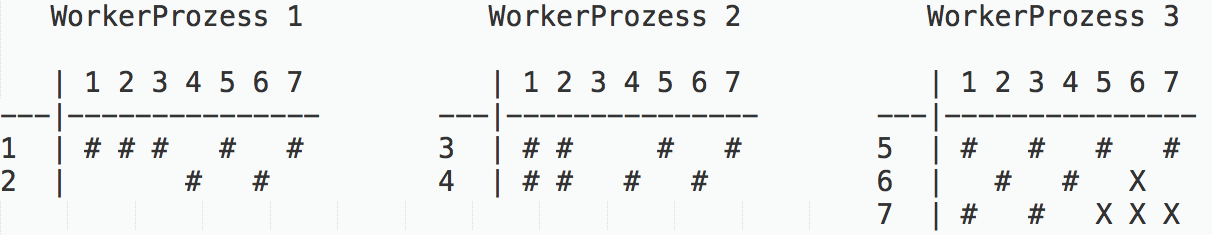
\includegraphics[width=0.9\columnwidth]{Raster_3} 
	\caption[Cluster-Prozess: Worker-Prozess: Nicht-Rechteck-Figuren]{Worker-Prozesse identifizieren Nicht-Rechteck-Figuren}
\end{figure}

Wenn ein Rechteck in einem Teil-Raster zu einem Rand der Teil-Rasters reicht und an diesem Rand im gesamten Raster ein weiteres Raster angrenzt, so könnte die Figur im angrenzenden Teil-Raster fortgesetzt werden. In diesem Fall ist also durch das Verarbeiten des Teil-Rasters keine Aussage darüber möglich, ob es sich um ein tatsächlich um ein Rechteck handelt. Entsprechende Rechtecke (Im Weiteren als potentielle Rechtecke) werden in der folgenden Grafik als \textit{?} gekennzeichnet.\\
Das Ergebnis der Abarbeitung der Teil-Raster in den Worker-Prozessen sieht also wie folgt aus:

\begin{figure}[h]
	\centering 
	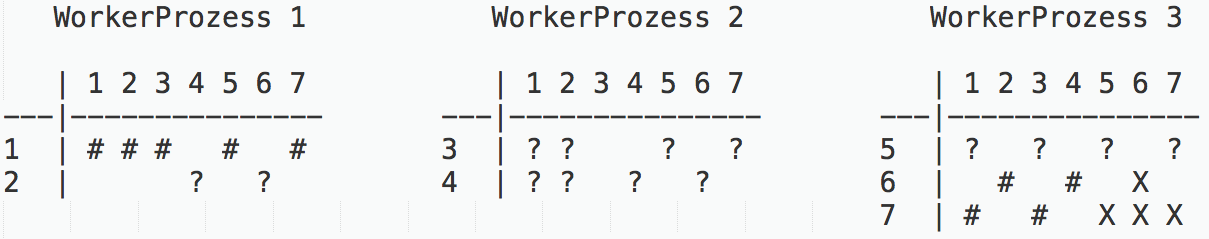
\includegraphics[width=0.9\columnwidth]{Raster_4} 
	\caption[Cluster-Prozess: Worker-Prozess: Rechtecke und potentielle Rechtecke]{Worker-Prozesse identifizieren Rechtecke und potentielle Rechtecke}
\end{figure}

Nach dem Verarbeiten der Teil-Raster durch die Worker-Prozesse, muss die finale Überprüfung der potentiellen Rechtecke vom Master-Prozess übernommen werden.

\begin{figure}[h]
	\centering 
	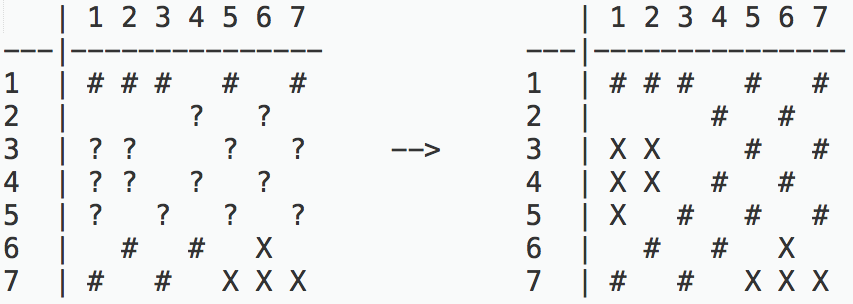
\includegraphics[width=0.7\columnwidth]{Raster_5} 
	\caption[Cluster-Prozess: Beispiel-Raster]{Ein Raster-Beispiel }
\end{figure}

Damit liegt dem Master-Prozess nun das vollständig überprüfte Raster vor. Die Einzelnen Rechtecke können nun dem Benutzer ausgegeben werden.\\

\textbf{Kommunikation und Ablauf im Cluster-Prozess }\\
Wie dabei Arbeits-Aufteilung und die Kommunikation zwischen den Prozessen verläuft, sei im Folgenden als BPMN-Diagramm dargestellt.\\

Der vollständige Code findet sich im Anhang. Die wesentlichen Funktionalitäten für den Master-Prozess finden sich dabei in dem Codeabschnitt, welcher ausgeführt wird, wenn der ausführende Prozess den Rang 0 hat und es mehr als einen Prozess gibt. Der Code für die Worker-Prozesse findet sich im Abschnitt, der ausgeführt wird, wenn der Rang des Prozesses nicht 0 ist.\\

Die Funktionalität zum Ermitteln der Rechtecke, wird im Kapitel 2.4 näher beschrieben. Nach welchem Prinzip die Zeitmessung erfolgen, wird in Kapitel 3.1 beschrieben.

\pagebreak

\begin{figure}[h]
	\centering 
	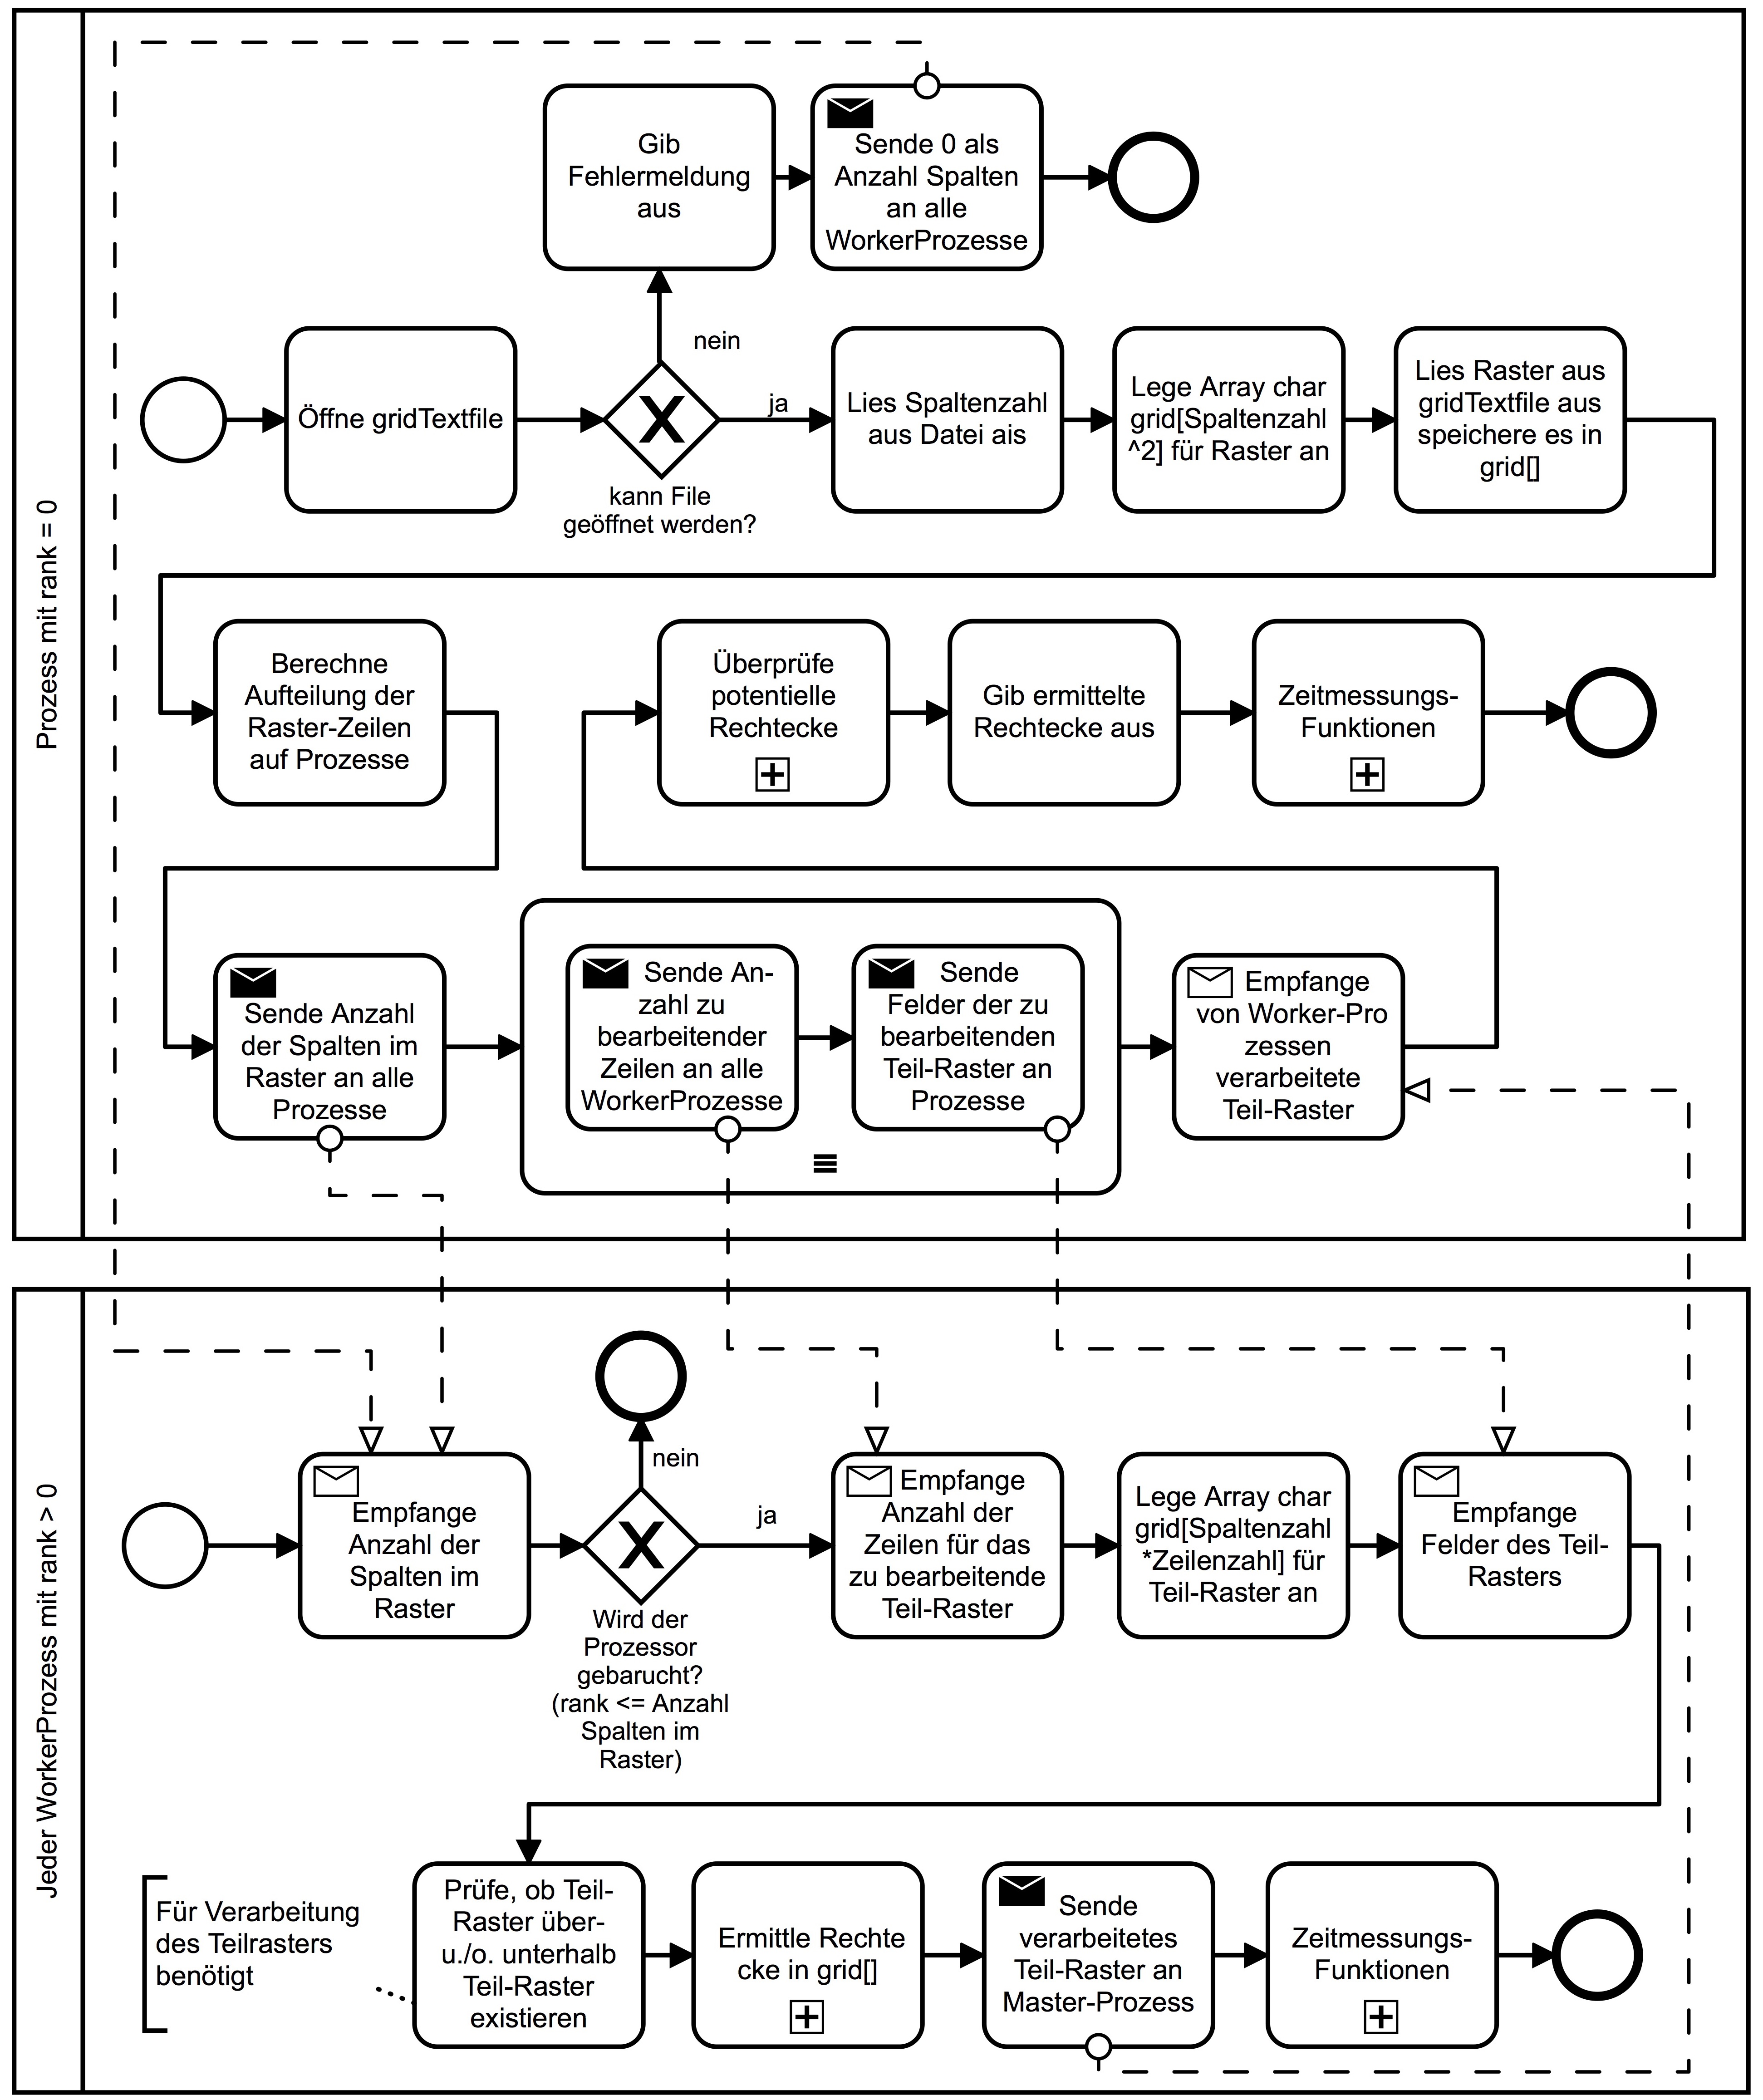
\includegraphics[width=1\columnwidth]{Diag_3f} 
	\caption[Funktionalität von \textit{pixCheckTangle.c} Cluster-Prozess]{Ablauf des Cluster-Prozesses von \textit{pixCheckTangle.c} dargestellt als BPMN-Diagramm }
	
\end{figure}



\subsection{pixCheckTangle: Funktion für das Abarbeiten eines (Teil-)Rasters}

Im Wesentlichen folgt das Vorgehen für die Unterscheidung zwischen Rechtecken und Nicht-Rechteck-Figuren dem folgenden Prinzip:

\begin{enumerate}[noitemsep]
	\item Erkenne Spalten-Reichweite der betrachteten Figur anhand der erster Zeile
	\item Ist In Zeile über der Figur innerhalb der Spalten-Reichweite ein Feld schwarz, ist die Figur kein Rechteck
	\item Enthält eine Zeile unterhalb der ersten innerhalb der Spalten-Reichweite der Figur schwarze und weiße Felder, ist die Figur kein Rechteck
	\item Grenzt an eine schwarze Zeile der Figur (von Spalten-Reichweite eingegrenzt) ein schwarzes Feld, ist die Figur kein Rechteck
\end{enumerate}
Zusätzlich ist dabei zu berücksichtigen, ob es sich bei einem erkannten Rechteck, wie weiter oben beschrieben, nur um ein potentielles Rechteck ist.\\
Die Implementierung der Funktion folgt danach dem folgenden, als Pseudo-Code dargestellten Algorithmus:\\

\begin{algorithm}[H]

	\KwData{$Raster$, $InfoZuAngenzedeTeilraster$}
	\KwResult{RasterVerarbeitet }
	\ForEach{$Feld$ in $Raster$ zeilenweise gelesen}{
		\If{$Feld$ ist Schwarz und nicht markiert}{
			$FigurIstRechteck \leftarrow wahr;$\\ 
			$startZeile \leftarrow aktuelle Zeile;$\\
			$startSpalte \leftarrow aktuelle Spalte;$\\
			$endeZeile \leftarrow aktuelle Zeile;$\\
			$endeSpalte \leftarrow$ Spalte von letzem $Feld$ in $startZeile$, das mit aktuellem $Feld$ zusammenhängt$;$\\
			\uIf{In Zeile über $startZeile$ im Bereich von $startSpalte$ bis $endeSpalte$ ist ein schwarzes Feld}{
				$FigurIstRechteck \leftarrow falsch;$\\
			}
			\Else{
				$RechteckGeprueft \leftarrow falsch;$\\
				\While{ $FigurIstRechteck $ und nicht $RechteckGeprueft$}{
					
					
					\uIf{Zeile unter $endeZeile$ enthält schwarze und weiße Felder}{
						$FigurIstRechteck \leftarrow falsch;$\\
				     }
				    \Else {
				    	\uIf{Zeile unter $endeZeile$ enthält nur schwarze Felder}{
				    		\uIf{In Zeile unter $endeZeile$ ist feld links von $startSpalte$ oder/und rechts $endeSpalte$ von schwarz}{
				    			$FigurIstRechteck \leftarrow falsch;$\\
				    		}
				    		\Else{
				    			$endeZeile \leftarrow endeZeile +1;$\\
				    		}
				    	}
				    	\Else{
				    		$RechteckGeprueft \leftarrow wahr;$\\
				    	}
				    }
				}
			}
		\uIf{$FigurIstRechteck$}{
			\uIf{$Figur$ liegt an Raster-Rand, der an weiterem Teil-Raster angrenzt}{
				Markiere alle schwarzen $Felder$ innerhalb der Reichweite, die von $startZeile$,$endeZeile$,$startSpalte$ und $endeSpalte$ aufgespannt wird als potentielles Rechteck-Feld;
			}
			\Else{
				Markiere alle schwarzen $Felder$ innerhalb der Reichweite, die von $startZeile$,$endeZeile$,$startSpalte$ und $endeSpalte$ aufgespannt wird als Rechteck-Feld;
			}
		}
		\Else{
			Markiere alle schwarzen $Felder$ innerhalb der Reichweite, die von $startZeile$,$endeZeile$,$startSpalte$ und $endeSpalte$ aufgespannt wird als Nicht-Rechteck-Feld;
		}
		}
	}	
\end{algorithm}\
\\
Der Code für die Funktionalität findet sich im Anhang im Programm \textit{pixCheckTangle.c} in der Funktion \textit{processSubgrid}.

\subsection{pixCheckTangle: Funktion für das Festlegen potentieller Rechtecke}

Für die Funktion zum Überprüfen der potentiellen Rechtecke, sobald die Worker-Prozesse die Teil-Raster abgearbeitet haben, wird die im Folgenden per Pseudo-Code beschriebene Vorgehensweise angewandt. Die Kernidee ist dabei nur noch Stichprobenartige Prüfungen zu machen, anstatt die Schritte aus dem oben aufgezeigte Prozess zu wiederholen. 

\begin{algorithm}[H]
	
	\KwData{$Raster$,$zuPruefendeZeile$ $InfoZuRasterumbrueche$}
	\KwResult{RasterVerarbeitet }
	\For{Jedes schwarze Feld in $zuPruefendeZeile$ mit Markierung = potentielles-Rechteck-Feld}{
		$startZeile \leftarrow aktuelle Zeile;$\\
		$startSpalte \leftarrow aktuelle Spalte;$\\
		$endeZeile \leftarrow aktuelle Zeile;$\\
		$endeSpalte \leftarrow$ Spalte von letzem $Feld$ in $startZeile$, das mit aktuellem $Feld$ zusammenhängt$;$\\
		\uIf{$zuPruefendeZeile$ ist Zeile oberhalb von Umbruch}{
			\uIf{In Zeile oberhalb $startZeile$ ist in Reichweite von $startSpalte$ bis $endeSpalte$ mindestens ein schwarzes Feld} {
				$zeilenMarker \leftarrow $ MIN(End-Zeile der Figur, Zeile vor folgendem Teil-Raster-Umbruch) $;$\\
				Markiere alle schwarzen $Felder$ innerhalb der Reichweite, die von $startZeile$,$zeilenMarker$,$startSpalte$ und $endeSpalte$ aufgespannt wird als Nicht-Rechteck-Feld;\\
				Fahre bei Feld nach der $endeSpalte$ fort.
			}
		}
		\uIf{hinter $zuPruefendeZeile$ folgt min 1 Teil-Raster-Umbruch}{
			\While{Ein Teilraster-Bruch folgt}{
				\uIf{Figur setzt unter Teilraster-Bruch fort}{
					\uIf{In erster Zeile nach Teilraster-Bruch ist die Laenge der Figur ungleich nicht mit der bisherigen Spalten-Reichweite}{
					$FigurIstRechteck \leftarrow falsch;$\\
					}
				}
			}
			$startZeile \leftarrow $ Anfang der Figur$;$\\
			\uIf{$FigurIstRechteck$}{
				$zeilenMarker \leftarrow $ Ende der Figur$;$\\
				Markiere alle schwarzen $Felder$ innerhalb der Reichweite, die von $startZeile$,$zeilenMarker$,$startSpalte$ und $endeSpalte$ aufgespannt wird als Rechteck-Feld;\\
				Fahre bei Feld nach der $endeSpalte$ fort.
			}
			\Else {
				$zeilenMarker \leftarrow $Letzte Zeile in der Rechteck-Bedingug fuer Figur erfuellt war$;$\\
				Markiere alle schwarzen $Felder$ innerhalb der Reichweite, die von $startZeile$,$zeilenMarker$,$startSpalte$ und $endeSpalte$ aufgespannt wird als Nicht-Rechteck-Feld;\\
				Fahre bei Feld nach der $endeSpalte$ fort.
			}
			
		}
		\Else{
			$zeilenMarker \leftarrow $ Ende der Figur$;$\\
			Markiere alle schwarzen $Felder$ innerhalb der Reichweite, die von $startZeile$,$zeilenMarker$,$startSpalte$ und $endeSpalte$ aufgespannt wird als Rechteck-Feld;\\
			Fahre bei Feld nach der $endeSpalte$ fort.
		}
	}
\end{algorithm}\

Der Code für die Funktionalität findet sich im Anhang im Programm \textit{pixCheckTangle.c} in der Funktion \textit{checkPotentialRectangle}.

\section{Messungen}
\subsection{Vorgehen beim Messen}

Für die Ermittlung des Speedups sollen Zeitmessungen durchgeführt werden. Da ein großer Anteil der Laufzeit für die Netzwerkkommunikation benötigt wird, soll hier zunächst eine Vorüberlegung angestellt werden, wie die Netzwerk-Kommunikation aus der Ausführungszeit herauszurechnen ist. \\Die Folgende schematische Darstellung zeigt die von den einzelnen Prozessen benötigte Zeit, in einem Cluster-Prozess mit 3 Worker-Prozessen.

\begin{figure}[h]
	\centering 
	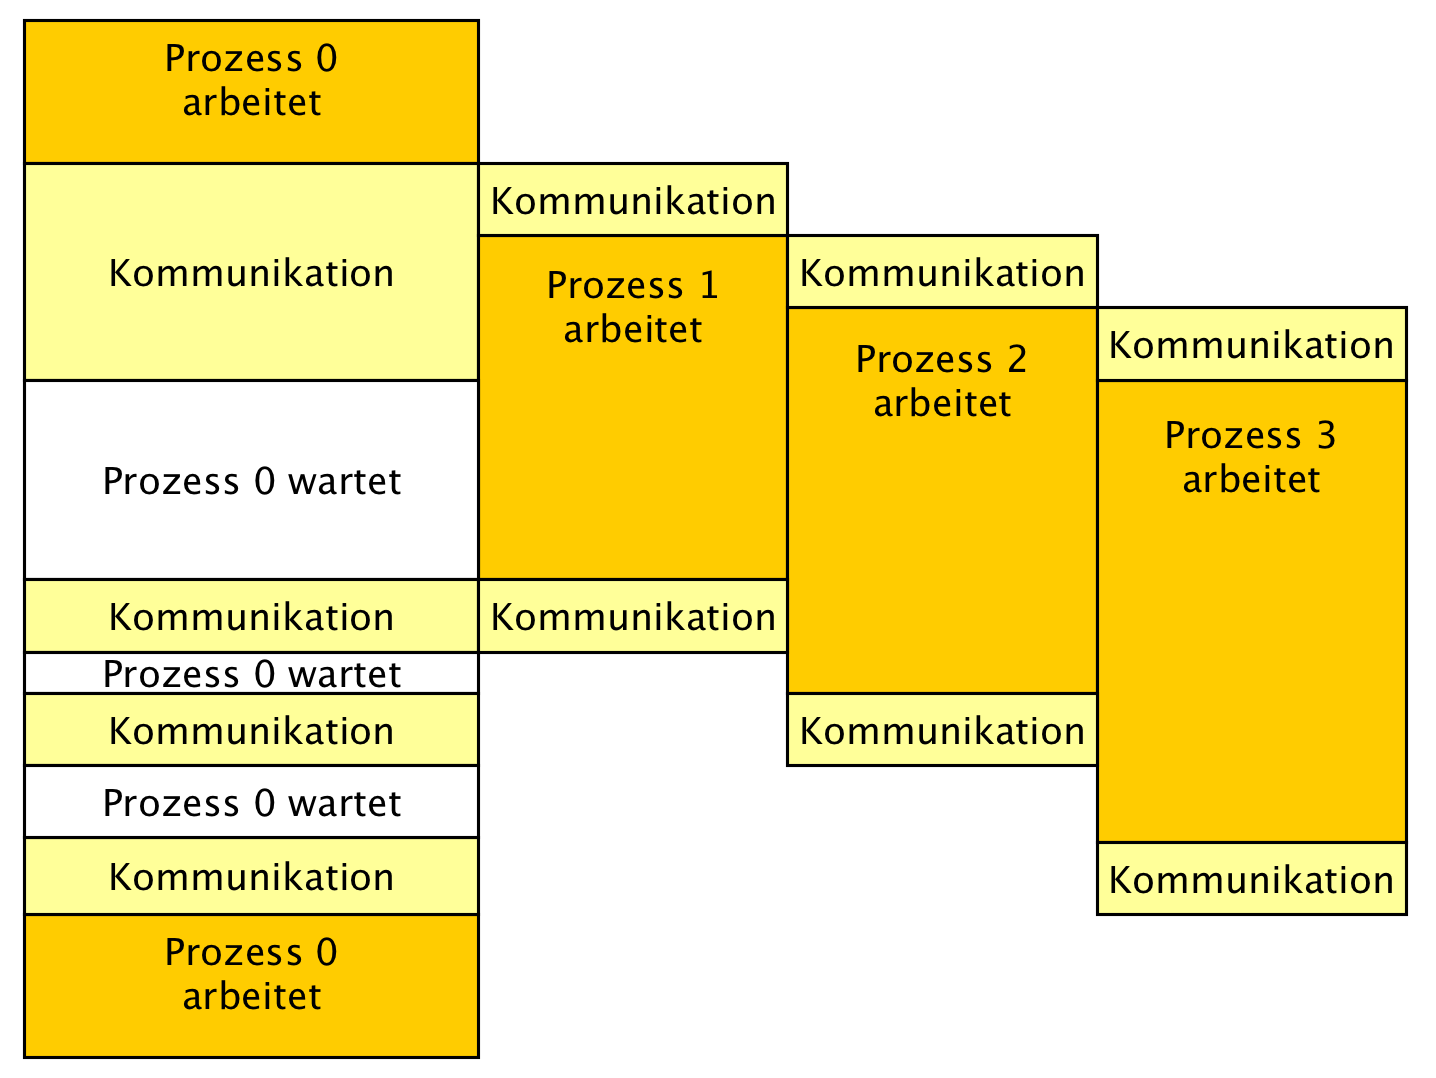
\includegraphics[width=0.5\columnwidth]{Time_1} 
	\caption[Skizze: Zeitbedarf mit Netzwerkkommunikation]{Skizze: Zeitbedarf mit Netzwerkkommunikation }
	
\end{figure}

Nimmt man hierbei an, dass die Netzwerkkommunikation keine Zeiteinheiten kostet, so erhält man näherungsweise die folgende schematische Darstellung.

\begin{figure}[h]
	\centering 
	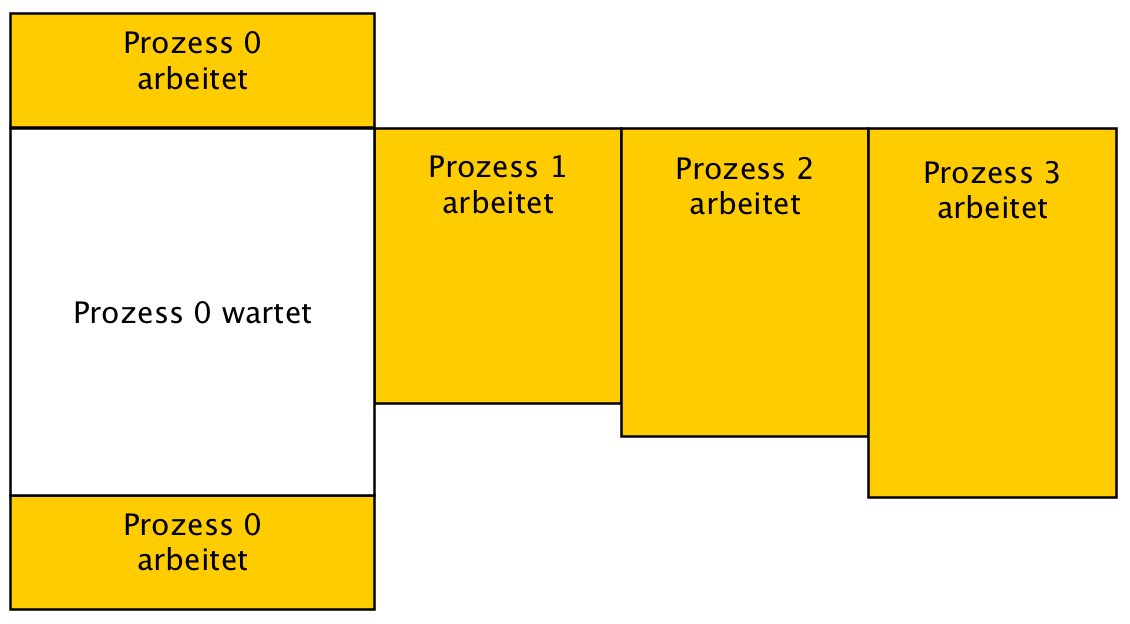
\includegraphics[width=0.5\columnwidth]{Time_2} 
	\caption[Skizze: Zeitbedarf ohne Netzwerkkommunikation]{Skizze: Zeitbedarf ohne Netzwerkkommunikation}
	
\end{figure}

Daraus geht hervor, dass sich die zu messende Zeit unter Ausschluss der Netzwerkkommunikation näherungsweise aus der von Prozess 0 benötigten aktiven Arbeitszeit und der benötigten Arbeitszeit, des am längsten laufenden Worker-Prozesses zusammensetzt.\\
Die Zeit-Messungen werden im Code mittels \textbf{MPI\_Wtime()}-Befehl realisiert. Zum ermitteln der maximalen Arbeitszeit aller Worker-Prozesse wird im Anschluss an die eigentliche Programm-Ausführung der \textbf{MPI\_Reduce()}-Befehl genutzt.\\
Die Resultate der Zeitmessungen im Code werden mittels der Funktion \textit{writeTimeToFile} in eine Datei geschrieben. 
Für die Ausführung von mehren Messreihen in einem Lauf werden die folgenden hilfs-Skripte/Programme verwendet. Diese sind im Anhang einzusehen.\\
\begin{itemize}[noitemsep] % [noitemsep] removes whitespace between the items for a compact look
	\item \textit{hostfileGenerator.c}: Generiert eine hostfile-Datei mit n Prozessoren.
	\item \textit{bsCreateHostfiles.sh}: ruft \textit{hostfileGenerator.c} auf, um mehrere  hostfiles zu erzeugen.
	\item \textit{bsRunGridTest.sh}: Ruft \textit{pixCheckTangle} per MPI für eine Raster-Datei und mehre Prozesse auf.
\end{itemize}

Gemessen werden:
\begin{itemize}[noitemsep] % [noitemsep] removes whitespace between the items for a compact look
	\item Laufzeit mit und ohne Netzwerkkommunikation
	\item Für Raster mit \textit{n=\{100/1000/10000\}} Feldern
	\item Pro Rastergröße: Messungen mit je \textit{p=\{1,2,..50\}} Prozessen.
	\item Pro Rastergröße und Prozess-Anzahl: drei verschiedene Probleminstanzen 
	\subitem - Alle Felder Weiß
	\subitem - Alle Felder Schwarz
	\subitem - Schachbrett-Raster
\end{itemize}

Jede Messung wird drei mal durchgeführt. Als Messwert wird der daraus gebildete Mittelwert betrachtet.

\subsection{Messergebnisse}


\subsection{Interpretation der Messergebnisse}



\section{Fazit}


\subsection{Einschätzung des Nutzens einer Parallelisierung}


\subsection{Mögliche Optimierungen}

\section{bla}

A statement requiring citation \cite{Figueredo:2009dg}.

\lipsum[1-3] % Dummy text

Some mathematics in the text: $\cos\pi=-1$ and $\alpha$.
 
%----------------------------------------------------------------------------------------
%	METHODS
%----------------------------------------------------------------------------------------

\section{Methods}

\lipsum[5] % Dummy text

\begin{enumerate}[noitemsep] % [noitemsep] removes whitespace between the items for a compact look
\item First item in a list
\item Second item in a list
\item Third item in a list
\end{enumerate}

%------------------------------------------------

\subsection{Paragraphs}

\lipsum[6] % Dummy text

\paragraph{Paragraph Description} \lipsum[7] % Dummy text

\paragraph{Different Paragraph Description} \lipsum[8] % Dummy text

%------------------------------------------------

\subsection{Math}

\lipsum[4] % Dummy text

\begin{equation}
\cos^3 \theta =\frac{1}{4}\cos\theta+\frac{3}{4}\cos 3\theta
\label{eq:refname2}
\end{equation}

\lipsum[5] % Dummy text

\begin{definition}[Gauss] 
To a mathematician it is obvious that
$\int_{-\infty}^{+\infty}
e^{-x^2}\,dx=\sqrt{\pi}$. 
\end{definition} 

\begin{theorem}[Pythagoras]
The square of the hypotenuse (the side opposite the right angle) is equal to the sum of the squares of the other two sides.
\end{theorem}

\begin{proof} 
We have that $\log(1)^2 = 2\log(1)$.
But we also have that $\log(-1)^2=\log(1)=0$.
Then $2\log(-1)=0$, from which the proof.
\end{proof}

%----------------------------------------------------------------------------------------
%	RESULTS AND DISCUSSION
%----------------------------------------------------------------------------------------

\section{Results and Discussion}

Reference to Figure~\vref{fig:gallery}. % The \vref command specifies the location of the reference

\begin{figure}[tb]
\centering 
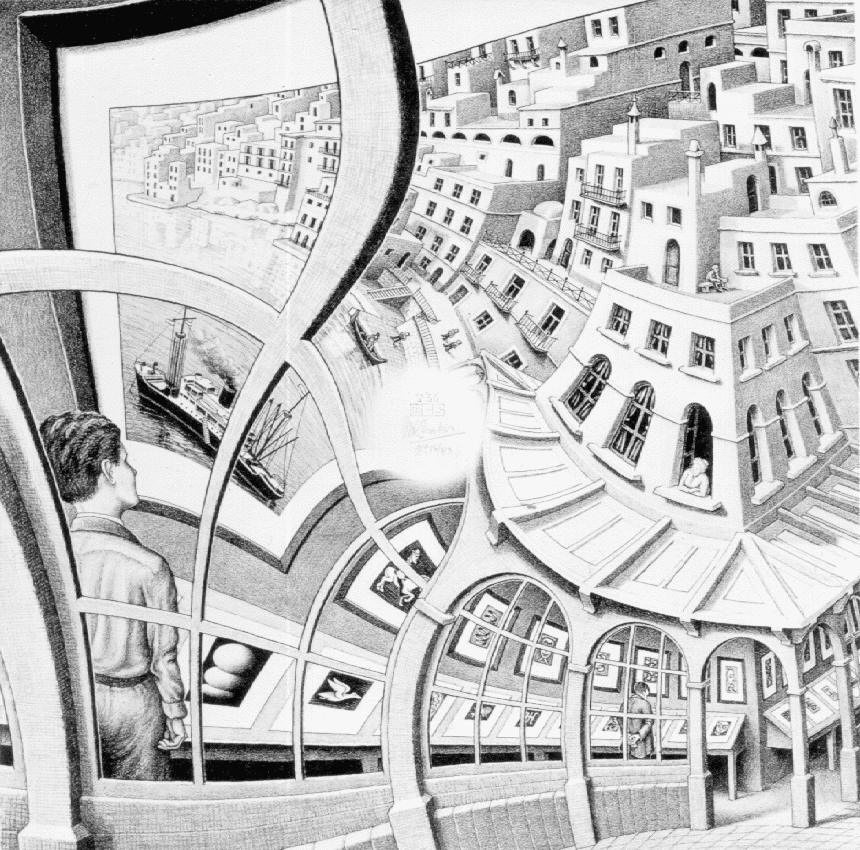
\includegraphics[width=0.5\columnwidth]{GalleriaStampe} 
\caption[An example of a floating figure]{An example of a floating figure (a reproduction from the \emph{Gallery of prints}, M.~Escher,\index{Escher, M.~C.} from \url{http://www.mcescher.com/}).} % The text in the square bracket is the caption for the list of figures while the text in the curly brackets is the figure caption
\label{fig:gallery} 
\end{figure}

\lipsum[10] % Dummy text

%------------------------------------------------

\subsection{Subsection}

\lipsum[11] % Dummy text

\subsubsection{Subsubsection}

\lipsum[12] % Dummy text

\begin{description}
\item[Word] Definition
\item[Concept] Explanation
\item[Idea] Text
\end{description}

\lipsum[12] % Dummy text

\begin{itemize}[noitemsep] % [noitemsep] removes whitespace between the items for a compact look
\item First item in a list
\item Second item in a list
\item Third item in a list
\end{itemize}

\subsubsection{Table}

\lipsum[13] % Dummy text

\begin{table}[hbt]
\caption{Table of Grades}
\centering
\begin{tabular}{llr}
\toprule
\multicolumn{2}{c}{Name} \\
\cmidrule(r){1-2}
First name & Last Name & Grade \\
\midrule
John & Doe & $7.5$ \\
Richard & Miles & $2$ \\
\bottomrule
\end{tabular}
\label{tab:label}
\end{table}

Reference to Table~\vref{tab:label}. % The \vref command specifies the location of the reference

%------------------------------------------------

\subsection{Figure Composed of Subfigures}

Reference the figure composed of multiple subfigures as Figure~\vref{fig:esempio}. Reference one of the subfigures as Figure~\vref{fig:ipsum}. % The \vref command specifies the location of the reference

\lipsum[15-18] % Dummy text

\begin{figure}[tb]
\centering
\subfloat[A city market.]{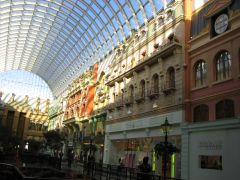
\includegraphics[width=.45\columnwidth]{Lorem}} \quad
\subfloat[Forest landscape.]{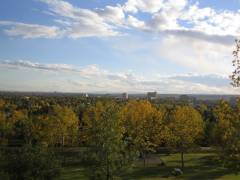
\includegraphics[width=.45\columnwidth]{Ipsum}\label{fig:ipsum}} \\
\subfloat[Mountain landscape.]{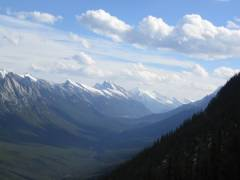
\includegraphics[width=.45\columnwidth]{Dolor}} \quad
\subfloat[A tile decoration.]{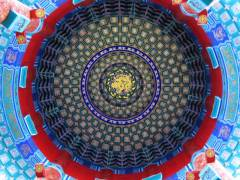
\includegraphics[width=.45\columnwidth]{Sit}}
\caption[A number of pictures.]{A number of pictures with no common theme.} % The text in the square bracket is the caption for the list of figures while the text in the curly brackets is the figure caption
\label{fig:esempio}
\end{figure}

%----------------------------------------------------------------------------------------
%	BIBLIOGRAPHY
%----------------------------------------------------------------------------------------

\renewcommand{\refname}{\spacedlowsmallcaps{References}} % For modifying the bibliography heading

\bibliographystyle{unsrt}

\bibliography{sample.bib} % The file containing the bibliography

%----------------------------------------------------------------------------------------

\end{document}